% vim: set ts=2 sw=2 noet spell:

\chapter{Theory}

\begin{figure}
	\centering
	\resizebox{\linewidth}{!}{
		\documentclass[tikz]{standalone}

\usepackage{roboto}
\usepackage{roboto-mono}
\usepackage{tikz}        % Pretty drawings
\usepackage{tikz-3dplot} % More dimensions!
\usetikzlibrary{
	external,
	calc,
	positioning,
	backgrounds,
	decorations.pathreplacing,
	calligraphy,
	decorations.markings,
	matrix,
	arrows,
	patterns,
}
\pgfdeclarelayer{background}
\pgfdeclarelayer{foreground}
\pgfsetlayers{background,main,foreground}

\begin{document}
\documentclass[tikz]{standalone}

\usepackage{roboto}
\usepackage{roboto-mono}
\usepackage{tikz}        % Pretty drawings
\usepackage{tikz-3dplot} % More dimensions!
\usetikzlibrary{
	external,
	calc,
	positioning,
	backgrounds,
	decorations.pathreplacing,
	calligraphy,
	decorations.markings,
	matrix,
	arrows,
	patterns,
}
\pgfdeclarelayer{background}
\pgfdeclarelayer{foreground}
\pgfsetlayers{background,main,foreground}

\begin{document}
\documentclass[tikz]{standalone}

\usepackage{roboto}
\usepackage{roboto-mono}
\usepackage{tikz}        % Pretty drawings
\usepackage{tikz-3dplot} % More dimensions!
\usetikzlibrary{
	external,
	calc,
	positioning,
	backgrounds,
	decorations.pathreplacing,
	calligraphy,
	decorations.markings,
	matrix,
	arrows,
	patterns,
}
\pgfdeclarelayer{background}
\pgfdeclarelayer{foreground}
\pgfsetlayers{background,main,foreground}

\begin{document}
\include{tikz/overview.tex}
\end{document}

\end{document}

\end{document}

	}
	\caption{
		Block diagram for a general wireless communication system with annotated signal names. Frequency domain representations of signals use the uppercase symbol of their respective time domain name.
		\label{fig:notation}
	}
\end{figure}

In this section we will briefly give the mathematical background required by the modulation schemes used in the project. The notation used is summarised in figure \ref{fig:notation}. For conciseness encoding schemes and (digital) signal processing calculations are left out and discussed later. Thus for this section \(m_e = m\).

%% TODO: Par on notation m(n) = m(nT) = discrete time

%% TODO: A section on maths?
% \section{Signal space and linear operators}

\section{Quadrature amplitude modulation (\(M\)-ary QAM)}

\begin{figure}
	\centering
	\resizebox{\linewidth}{!}{
		% vim: set ts=2 sw=2 noet:

\begin{circuitikz}[
	]
	\matrix [
		row sep = 5mm, column sep = 7mm,
		nodes = {
			align = center,
			fill = white,
		},
	] {
		& \coordinate (vmi);
			& \node[twoportshape] (B2Li) {};
			&
			& \coordinate (mi);
			&
			& \node[mixer] (Mi) {};
			& \coordinate (si);
			\\
		\node[] (M) {\(m(n)\)};
			& \node[twoportshape] (BSp) {};
			&
			&
			& \node[twoportshape] (H) {};
			& \node[oscillator] (OSC) {};
			& \coordinate (phii);
			& \node[adder] (SUM) {};
			& \node (S) {\(s(t)\)};
			\\
		&&&& \coordinate (phiq);
			\\[-3mm]
		& \coordinate (vmq);
			& \node[twoportshape] (B2Lq) {};
			& \coordinate (mq);
			& \node[mixer] (Mq) {};
			&
			&
			& \coordinate (sq);
			\\
	};

	% Add missing lables
	\node at (H.center) {\large \(\mathcal{H}\)};
	\node at (B2Li.center) {\textsf{B2L}};
	\node at (B2Lq.center) {\textsf{B2L}};
	\node at (BSp) {\textsf{BSp}};

	% Add connections
	\begin{scope}[thick, -latex]
		\draw (M) -- (BSp.west);

		\draw (BSp.north) |- (B2Li.west);
		\draw (B2Li.east) -- (Mi.west);
		\draw (Mi.east) -| (SUM.north);

		\draw (BSp.south) |- (B2Lq.west);
		\draw (B2Lq.east) -- (Mq.west);
		\draw (Mq.east) -| (SUM.south);

		\draw (SUM.east) -- (S);

		\draw (OSC.east) -| (Mi.south);
		\draw (OSC.west) -- (H.east);
		\draw (H.south) -- (Mq.north);
	\end{scope}

	% Add signal labels
	\node[above right] at (vmi) {\(\vec{m}_i\)};
	\node[below right] at (vmq) {\(\vec{m}_q\)};

	\node[above] at (mi) {\(m_i(t)\)};
	\node[below] at (mq) {\(m_q(t)\)};

	\node[above right] at (phii) {\(\phi_i\)};
	\node[right, yshift = 1mm] at (phiq) {\(\phi_q\)};

	\node[above left] at (si) {\(s_i(t)\)};
	\node[below left] at (sq) {\(s_q(t)\)};

	% Draw digital signals
	\begin{scope}[font = \ttfamily\footnotesize, text = blue!70!white]
		\node[above = 1mm of M, xshift = 2mm] {\(\ldots 1100101\)};
		\node[above = 7mm of vmi, xshift = 3mm]
			{\(\overbracket[.8pt]{\,11\ldots 00\,}^{\sqrt{M} \text{ bits}}\)};
	\end{scope}

	% Draw analog waveform
	\begin{scope}[font = \ttfamily\tiny]
		\coordinate (O) at ($(mi)+(-2mm,10.5mm)$);

		\node[left, red!70!white, anchor = east, text width = 8mm, align = right]
			at ($(O) + (-2mm,0)$) {\(2^{\sqrt{M}}\) levels};

		\foreach \y in {-3mm,0,3mm} {
			\draw[gray, densely dotted] (O) ++(-2mm,\y) -- ++(22mm,0);
		}

		\draw[thick, draw = red!70!white] (O)
			-- ++(3mm,0) -- ++(0,-3mm) -- ++(3mm,0) -- ++(0,6mm)
			-- ++(3mm,0) -- ++(0,-3mm) -- ++(3mm,0) -- ++(0,-3mm)
			-- ++(3mm,0) -- ++(0,3mm)  -- ++(3mm,0);
	\end{scope}

	% Draw constellation diagram
	\begin{scope}
		\coordinate (O) at ($(S)+(-7mm,8mm)$);
		\draw[gray, -latex] (O) ++(-2mm,0) -- ++(12mm,0) node[right] {\tiny \(\phi_i\)};
		\draw[gray, -latex] (O) ++(0,-2mm) -- ++(0,12mm) node[above] {\tiny \(\phi_q\)};

		\node[
			circle, thick,
			minimum size = 3pt,
			inner sep = 0, outer sep = .8pt,
			draw = gray, fill = red!50!white
		] (P) at ($(O)+(5mm, 4mm)$) {};

		\node[gray, above right] at (P) {\tiny \(s\)};

		\draw[gray, densely dotted]
			(P) -- (P |- O)
			(P) -- (P -| O);
	\end{scope}


	% Background elements
	\begin{pgfonlayer}{background}
		\fill[left color = white, right color = blue!20, draw = white]
			($(B2Li.north) + (0,1.1)$) coordinate (D) rectangle ($(B2Lq.south) - (3,1)$);
		\fill[right color = white, left color = red!20, draw = white]
			($(B2Li.north) + (0,1.1)$) coordinate (A) rectangle ($(B2Lq.south) + (9,-1)$);

		\node[blue!50, anchor = south east, font = \ttfamily\bfseries, xshift = -4mm]
			at (D) {\bfseries\ttfamily Digital bits};
		\node[red!50, anchor = south west, font = \bfseries\ttfamily, xshift = 4mm]
			at (A) {Analog waveform};
	\end{pgfonlayer}
\end{circuitikz}

	}
	\caption{
		Block diagram of a \(M\)-ary QAM modulator.
		\label{fig:quadrature-modulation}
	}
\end{figure}

Quadrature amplitude modulation is a family of modern digital modulation methods, that use an analog carrier signal. The simple yet effective idea behind QAM is to encode extra information into an orthogonal carrier signal, thus increasing the number of bits sent per unit of time. A block diagram of the process is shown in figure \ref{fig:quadrature-modulation}.

%% TODO: Quick par on "we will dicusss M-Ary QAM, M is 2^something"

\subsection{Modulation of a digital message}

\paragraph{Bit splitter}

As mentioned earlier, quadrature modulation allows sending more than one bit per unit time. The first step to do it is to use a so called bit splitter, that converts the continuous bitstream \(m(n)\) into pairs of chunks of \(\sqrt{M}\) bits. The two bit vectors of length \(\sqrt{M}\), denoted by \(\vec{m}_i\) and \(\vec{m}_q\) in figure \ref{fig:quadrature-modulation}, are called in-phase and quadrature component respectively. The reason will become more clear later.

\paragraph{Binary to level converter}

%% TODO: explain why gray code

Both bit vectors \(\vec{m}_i, \vec{m}_q \in \{0,1\}^{\sqrt{M}}\) are sent through a binary to level converter. It's purpose is to reinterpret the bit vectors as a numbers, usually in gray code, and to convert them into analog waveforms, which we will denote with \(m_i(t)\) and \(m_q(t)\) respectively. Mathematically the binary to level converter can be described as:
\begin{equation}
	m_i(t) = \text{Level}(\vec{m}_i) \cdot p(t),
\end{equation}
i.e. a pulse function\footnote{Typically a root raised cosine to optimize for bandwidth.} \(p(t)\) scaled by the interpreted binary value, written here using a ``Level'' function. So at this point a level of each analog waveform is encodes \(\sqrt{M}\) bits per unit time, and there are two of such waveforms.


\paragraph{Mixer}

Having analog level signals, it is this now possible to mix them with radio frequency carriers. Because there are two waveforms, one might expect that two carrier frequencies are necessary, however this is not the case. The two component \(m_i(t)\) and \(m_q(t)\) are mixed with two different periodic signals \(\phi_i(t)\) and \(\phi_q(t)\) that have the same frequency \(\omega_c = 2\pi / T\). Why this is possible is explained in the next section.


\subsection{Orthogonality of carrier signals}

Before explaining how the two carrier signals are generated, we first need to discuss some important mathematical properties \(\phi_i\) and \(\phi_q\) need to have, in order to modulate two messages over the same frequency \(\omega_c\). The two carriers need to be \emph{orthonormal}\footnote{Actually orthogonality alone would be sufficient, however then the left side of \eqref{eqn:orthonormal-condition} would not equal 1, and an inconvenient factor would be introduced in many later equations.} to each other, mathematically this is expressed by the conditions
\begin{subequations} \label{eqn:orthonormal-conditions}
	\begin{align}
		\langle \phi_i, \phi_q \rangle
			&= \int_T \phi_i \phi_q^* \, dt
			= 0, \text{ and } \label{eqn:orthogonal-condition} \\
		\langle \phi_k, \phi_k \rangle
			&= \int_T \phi_k \phi_k^*  \,dt = 1,
			\text{ where } k \text{ is either } i \text{ or } q. \label{eqn:orthonormal-condition}
	\end{align}
\end{subequations}
Provided these rather abstract conditions, let's define a new signal 
\begin{equation}
	s = m_i\phi_i + m_q\phi_q.
\end{equation}
%% TODO: is this assumption correct?
Notice that assuming \(m_i\) and \(m_q\) are constant\footnote{This is an approximation assuming that the signal changes much slower relative to the carrier.} over the carrier's period \(T\),
\begin{align*}
	\langle s, \phi_i \rangle = \int_T s \phi_i^* \,dt
		&= \int m_i \phi_i \phi_i^* + m_q \phi_q \phi_i^* \,dt \\
		&= m_i \underbrace{\int_T \phi_i \phi_i^* \,dt}_{1}
			+ m_q \underbrace{\int_T \phi_q \phi_i^* \,dt}_{0} = m_i,
\end{align*}
which effectively means that it is possible to isolate a single component \(m_i(t)\) out of \(s(t)\). The same of course works with \(\phi_q\) as well resulting in \(\langle s, \phi_q \rangle = m_q\). Thus (remarkably) it is possible to send two signals on the same frequency, without them interfering with each other. Since each signal can represent one of \(\sqrt{M}\) values, by having two we obtain \(\sqrt{M} \cdot \sqrt{M} = M\) possible combinations.

A graphical way to see what is happening, is to observe a so called \emph{constellation diagram}. An example is shown in figure \ref{fig:qam-constellation} for \(M = 16\). The two carrier signals \(\phi_i\) and \(\phi_q\) can be understood as bases of a coordinate system.

\subsection{Construction of orthogonal carrier signals}


If \(\phi_i\) is a real valued signal (which is typical) it is possible to find a function the quadrature carrier using the \emph{Hilbert transform}:
\begin{equation}
	\hilbert g(t) = g(t) * \frac{1}{\pi t}
		= \frac{1}{\pi} \int_\mathbb{R} \frac{g(\tau)}{t - \tau} \,d\tau
		= \frac{1}{\pi} \int_\mathbb{R} \frac{g(t - \tau)}{\tau} \,d\tau,
\end{equation}
i.e. a linear operator that introduces a phase shift of \(\pi / 2\) over all frequencies. It is a known property of the Hilbert transform that given a real valued function \(g(t)\) then \(\langle g, \hilbert g \rangle = 0\).
In practice \(\phi_i(t) = \cos(\omega_c t)\) and \(\phi_q(t) = \hilbert \phi_i(t) = \sin(\omega_c t)\).  

\paragraph{Oscillator and phase shifter}

\begin{figure}
	\hfill
	\begin{subfigure}{.4\linewidth}
		% vim: set ts=2 sw=2 noet:
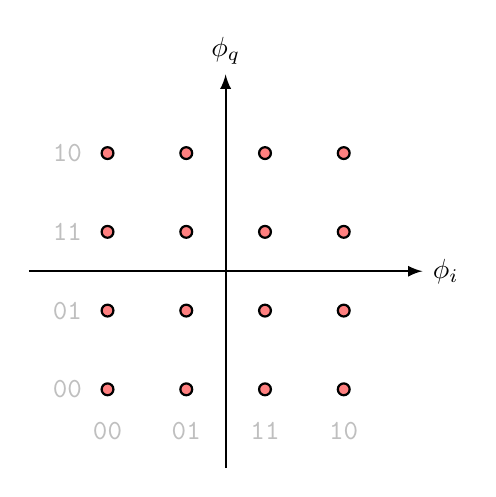
\begin{tikzpicture}[
		axis/.style = {
			thick, -latex, black,
		},
		star/.style = {
			draw = black, thick, fill = red!50,
			circle, outer sep = 1mm, inner sep = 0,
			minimum size = 1.5mm,
		},
	]
	\draw[axis] (-25mm,0) to (25mm,0) node[right] {\(\phi_i\)};
	\draw[axis] (0,-25mm) to (0,25mm) node[above] {\(\phi_q\)};

	\foreach \i in {0,1,...,3}{
		\foreach \q in {0,1,...,3}{
			\node[star] (s\i\q) at ({\i*10mm - 15mm},{\q*10mm - 15mm}) {};
		}
	}

	\foreach \i/\l in {0/00,1/01,2/11,3/10}{
		\node[lightgray, below = 3mm] at (s\i0) {\texttt{\l}};
		\node[lightgray, left = 2mm] at (s0\i) {\texttt{\l}};
	}
\end{tikzpicture}

		\caption{16-QAM\label{fig:qam-constellation}}
	\end{subfigure}
	\hfill
	\begin{subfigure}{.4\linewidth}
		\input{figures/tikz/psk-constellation}
		\caption{8-PSK\label{fig:psk-constellation}}
	\end{subfigure}
	\hfill
	\caption{
		Examples of constellation diagrams. Each dot represents a possible location for the complex amplitude of the passband signal.
	}
\end{figure}


\section{Phase shift keying (\(M\)-PSK)}

PSK is a popular modulation type for data transmission\cite{Meyer2011}. With a bipolar binary signal, the amplitude remains constant and only the phase will be changed with phase jumps of 180 degrees, which can be seen as a multiplication of the carrier signal with $\pm$ 1. That is alow known as binary phase shift keying.

% \begin{figure}
% 	% TODO: Better Image
% 	% https://sites.google.com/site/billmahroukelec675/bipolar-phase-shift-keying
% 	\includegraphics[width=5cm]{./image/BPSK2.png}
% \end{figure}

Two bits are modulated at ones with the same bandwidth as a 2-PSK so more informations are transmitted at the same time. \cite{Meyer2011}
%TODO: Image Signal Raum 
Most times there is noise and the points on the constellation diagram become a surface. 
If the surfaces overlap there will be a problem with decoding. 

\section{Chanel noise and fading}

\subsection{Geometric Model}


\subsection{Statistical Model}

%% TODO: write about advantage of statistical model instead of geometric

\paragraph{Continuous time model}

Continuous time small scale fading channel response.

time varying channel impulse response:
\begin{equation}
	h(t, \tau) = \sum_k c_k (t) \delta(\tau - \tau_k(t))
\end{equation}

received signal \(y = h * x\), i.e. convolution with channel model. 

\subsection{Time discretization of the model}

%% TODO: explain why

Assume \(x\) is a time discrete signal with and bandwidth \(W\), thus the pulse is sinc shaped
\begin{equation}
	x(t) = \sum_n x(n) \sinc(t/T - n)
\end{equation}
Ideal sampling at rate \(2W\) of \(y\) gives

\section{Receiver DSP chain}
